% Figure 1: the label hierarchy and the alternative decision routes.
%
% Build with analysis/figure1.py (or `python -m analysis`), never by hand:
% the counts come from figure1_defs.tex, which is generated from paper.labels.
% Nothing in this file may type a count out; tests/test_analysis_figure1.py
% fails the build if it does.
%
% Fonts are the ACM template's own, so the figure's type matches the paper's.
% Panel coordinates run 0-10 and are scaled once, which keeps the geometry
% readable while leaving the type at its true size.
%
% For D: the natural size is 15.4 x 7.0 cm (6.1 x 2.8 in), meant for figure*
% across both columns. Include it without a width key -- at 1:1 the labels sit
% at 8pt against the template's 9pt body. Forcing width=\textwidth enlarges
% them past the running text, and no single-column reduction leaves them
% legible; this figure carries too much to fit one column.
\documentclass[border=1pt]{standalone}
% Pinned so two builds produce the same bytes: pdfTeX derives the trailer /ID
% from the output path and the clock. The date half is pinned by
% SOURCE_DATE_EPOCH in analysis/figure1.py.
\ifdefined\pdftrailerid\pdftrailerid{}\fi
% SOURCE_DATE_EPOCH reaches latexmk but the standalone class does not honour it,
% so the timestamp is omitted outright instead. A figure whose bytes change on
% every rebuild cannot be committed, and this one is.
\ifdefined\pdfinfoomitdate\pdfinfoomitdate=1\fi

\usepackage[T1]{fontenc}
\usepackage[tt=false,type1=true]{libertine}
\usepackage[libertine]{newtxmath}
\usepackage{tikz}
\usetikzlibrary{arrows.meta,positioning}

% Generated by analysis/figure1.py from paper.labels -- do not edit.
% Every number Figure 1 prints is defined here so that none is typed
% into the drawing by hand.
\newcommand{\NumStates}{17}
\newcommand{\NumCombinations}{120}
\newcommand{\NumInvalid}{103}
\newcommand{\NumTimelines}{4}
\newcommand{\NumQualities}{3}
\newcommand{\NumPromiseLabels}{2}
\newcommand{\NumTimelineLabels}{5}
\newcommand{\NumEvidenceLabels}{3}
\newcommand{\NumQualityLabels}{4}


% Okabe--Ito accents plus pale tints: distinguishable under common colour-
% vision deficiencies, while labels and marker shapes preserve the meaning in
% greyscale.
\definecolor{ink}{HTML}{273746}
\definecolor{muted}{HTML}{64727D}
\definecolor{panelblue}{HTML}{F1F7FB}
\definecolor{panelgrey}{HTML}{F6F7F8}
\definecolor{blue}{HTML}{0072B2}
\definecolor{bluefill}{HTML}{DCEEF8}
\definecolor{sky}{HTML}{56B4E9}
\definecolor{skyfill}{HTML}{E6F4FA}
\definecolor{teal}{HTML}{009E73}
\definecolor{tealfill}{HTML}{DDF2EB}
\definecolor{vermillion}{HTML}{D55E00}
\definecolor{vermillionfill}{HTML}{F9E6DC}
\definecolor{purple}{HTML}{8B6BB1}
\definecolor{purplefill}{HTML}{EEE8F5}

\tikzset{
  panel/.style = {rounded corners=5pt, draw=muted!42, line width=0.38pt},
  card/.style = {rounded corners=3pt, line width=0.55pt, align=center,
                 inner sep=4pt, text=ink},
  field/.style = {card, draw=blue, fill=bluefill},
  terminal/.style = {card, draw=teal, fill=tealfill},
  branch/.style = {card, draw=sky!80!blue, fill=skyfill},
  base/.style = {card, draw=blue, fill=bluefill, minimum width=5.2cm},
  invalid/.style = {card, draw=vermillion, fill=vermillionfill,
                    minimum width=2.15cm, minimum height=2.15cm},
  projection/.style = {card, draw=blue, fill=bluefill,
                       minimum width=2.35cm, minimum height=2.15cm},
  decoder/.style = {card, draw=teal, fill=tealfill,
                    minimum width=2.35cm, minimum height=2.15cm},
  chip/.style = {rounded corners=5pt, draw=purple, fill=purplefill,
                 line width=0.4pt, inner xsep=3pt, inner ysep=1.5pt,
                 font=\scriptsize, text=ink},
  statusbad/.style = {rounded corners=5pt, draw=vermillion,
                      fill=vermillionfill, text=vermillion!75!black,
                      font=\bfseries\scriptsize, inner xsep=4pt,
                      inner ysep=1.6pt},
  statusgood/.style = {rounded corners=5pt, draw=teal, fill=tealfill,
                       text=teal!65!black, font=\bfseries\scriptsize,
                       inner xsep=4pt, inner ysep=1.6pt},
  edgelabel/.style = {text=muted, fill=white, rounded corners=2pt,
                      inner sep=1.4pt, font=\scriptsize},
  note/.style = {text=ink, align=center},
  aside/.style = {text=muted, align=center, font=\scriptsize},
  title/.style = {text=ink, anchor=west, font=\bfseries\small},
  subtitle/.style = {text=muted, anchor=west, font=\scriptsize},
  route/.style = {draw=ink!72, line width=0.48pt,
                  -{Stealth[length=3pt,width=2.4pt]}},
}

\begin{document}
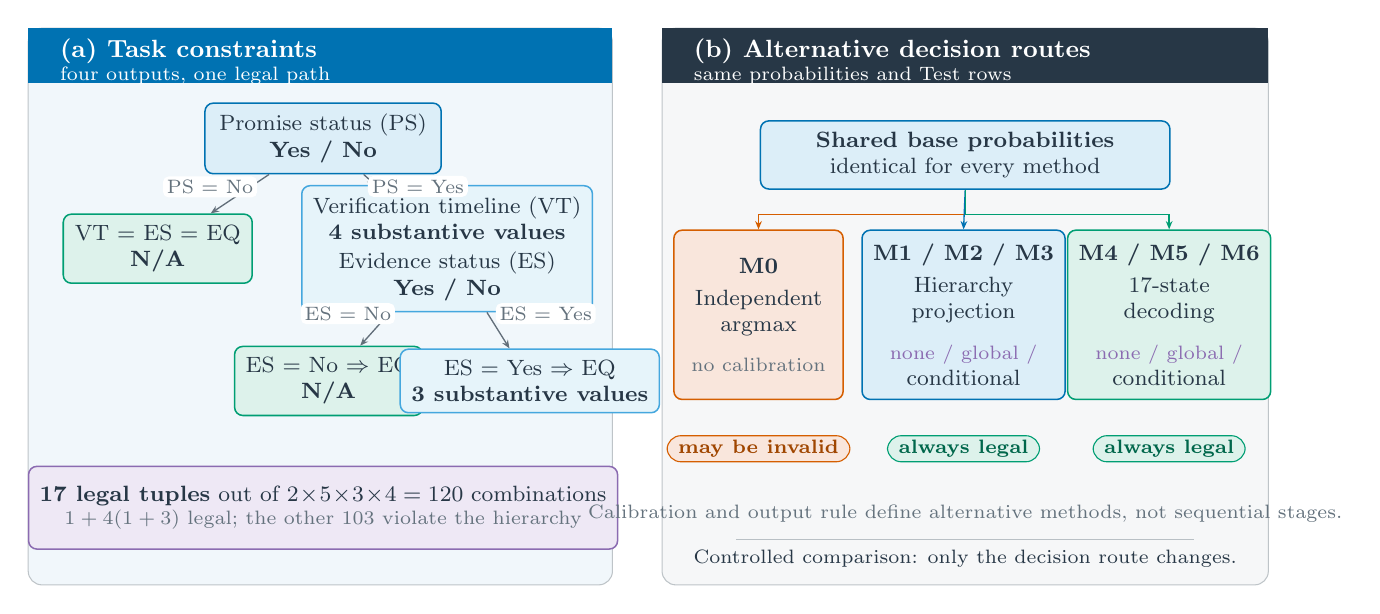
\begin{tikzpicture}[scale=0.70, font=\footnotesize]

% ---------------------------------------------------------------- panel (a)
\filldraw[panel, fill=panelblue] (-0.35,0.25) rectangle (10.25,10.35);
\fill[blue] (-0.35,9.35) rectangle (10.25,10.35);
\node[title, text=white] at (0.05,9.93) {(a) Task constraints};
\node[subtitle, text=white!88] at (0.05,9.48)
  {four outputs, one legal path};

\node[field, minimum width=3.0cm] (ps) at (5.0,8.35)
  {Promise status (PS)\\\textbf{Yes / No}};
\node[terminal, minimum width=2.4cm] (psno) at (2.0,6.35)
  {VT = ES = EQ\\\textbf{N/A}};
\node[branch, minimum width=3.2cm] (psyes) at (7.25,6.35)
  {Verification timeline (VT)\\\textbf{\NumTimelines{} substantive values}\\[1pt]
   Evidence status (ES)\\\textbf{Yes / No}};

\draw[route] (ps) -- (psno);
\draw[route] (ps) -- (psyes);
\node[edgelabel] at (2.95,7.47) {PS = No};
\node[edgelabel] at (6.72,7.48) {PS = Yes};

\node[terminal, minimum width=2.35cm] (esno) at (5.1,3.95)
  {ES = No $\Rightarrow$ EQ\\\textbf{N/A}};
\node[branch, minimum width=2.45cm] (esyes) at (8.75,3.95)
  {ES = Yes $\Rightarrow$ EQ\\\textbf{\NumQualities{} substantive values}};

\draw[route] (psyes) -- (esno);
\draw[route] (psyes) -- (esyes);
\node[edgelabel] at (5.45,5.17) {ES = No};
\node[edgelabel] at (9.04,5.17) {ES = Yes};

\node[card, draw=purple, fill=purplefill, minimum width=7.0cm,
      minimum height=1.05cm] at (5.0,1.65)
  {\textbf{\NumStates{} legal tuples} out of
   $\NumPromiseLabels\!\times\!\NumTimelineLabels\!\times\!
    \NumEvidenceLabels\!\times\!\NumQualityLabels
    = \NumCombinations$ combinations\\[-1pt]
   \scriptsize\color{muted}$1+\NumTimelines(1+\NumQualities)$ legal;
   the other \NumInvalid{} violate the hierarchy};

% ---------------------------------------------------------------- panel (b)
\begin{scope}[shift={(11.5, 0)}]
\filldraw[panel, fill=panelgrey] (-0.35,0.25) rectangle (10.65,10.35);
\fill[ink] (-0.35,9.35) rectangle (10.65,10.35);
\node[title, text=white] at (0.05,9.93) {(b) Alternative decision routes};
\node[subtitle, text=white!82] at (0.05,9.48)
  {same probabilities and Test rows};

\node[base] (base) at (5.15,8.05)
  {\textbf{Shared base probabilities}\\identical for every method};

\node[invalid] (mzero) at (1.4,5.15)
  {\textbf{M0}\\[2pt]Independent\\argmax\\[5pt]
   \scriptsize\color{muted}no calibration};
\node[projection] (mproj) at (5.12,5.15)
  {\textbf{M1 / M2 / M3}\\[2pt]Hierarchy\\projection\\[5pt]
   \scriptsize\color{purple}none / global /\\conditional};
\node[decoder] (mdecode) at (8.85,5.15)
  {\textbf{M4 / M5 / M6}\\[2pt]\NumStates-state\\decoding\\[5pt]
   \scriptsize\color{purple}none / global /\\conditional};

\draw[route, draw=vermillion] (base.south) -- ++(0,-0.45) -| (mzero.north);
\draw[route, draw=blue]       (base.south) -- (mproj.north);
\draw[route, draw=teal]       (base.south) -- ++(0,-0.45) -| (mdecode.north);

\node[statusbad]  at (1.4,2.72) {may be invalid};
\node[statusgood] at (5.12,2.72) {always legal};
\node[statusgood] at (8.85,2.72) {always legal};

\node[aside] at (5.15,1.55)
  {Calibration and output rule define alternative methods, not sequential stages.};
\draw[draw=muted!45, line width=0.4pt] (1.0,1.08) -- (9.3,1.08);
\node[note, font=\scriptsize] at (5.15,0.73)
  {Controlled comparison: only the decision route changes.};
\end{scope}

\end{tikzpicture}
\end{document}
